\section{Methods}

\subsection{Importance sampling}
\begin{itemize}
\item Importance sampling is a well known technique in the domain
  of statistics \cite{importanceSampling}. In case of ASE-Flux calculation a presampling of
  a sample point is done to figure out important areas
  inside the mesh. Important areas generate more rays for a
  particular sample point.
\item Importance sampling can increase the efficiency of Monte-Carlo-Simulations (reduce variance)
\end{itemize}

\subsection{Adaptive rays}
\begin{itemize}
\item Since most sample points behave in a good way, they don't need
  to be samlped with a high number of rays. Only some outliers have high Mean
  Squared Error, these need resampling.
\item MSE in formula: 
     \[f(\vec{r_0}) = \frac{1}{n} \sum_{i=1}^n g_i \]
     \[f^2(r_0) = \frac{1}{n} \sum_{i=1}^n g_i^2 \]
     \[MSE(r_0) = \sqrt{\frac{f^2(r_0) - f(r_0)^2}{n}}\]
\item Dependant on a $MSE$-threshold and the $MSE$ value
  of the sample, the number of rays per sample point 
  will be increased to a maximum number.
\item Thus not every sample point needs to be sampled
  with a high number of rays to obtain high precision.
  Only sample points with $MSE(r_0) \quad \textgreater \quad MSE$-threshold need
  resampling. This saves a lot of calculation time.
\item By decresing the MSE threshold (increasing precision), the runtime increses because
  of a higher number of rays per sample point. It could also happen, that the maximum number
  of rays are not enough to reach the given MSE threshold.
\end{itemize}
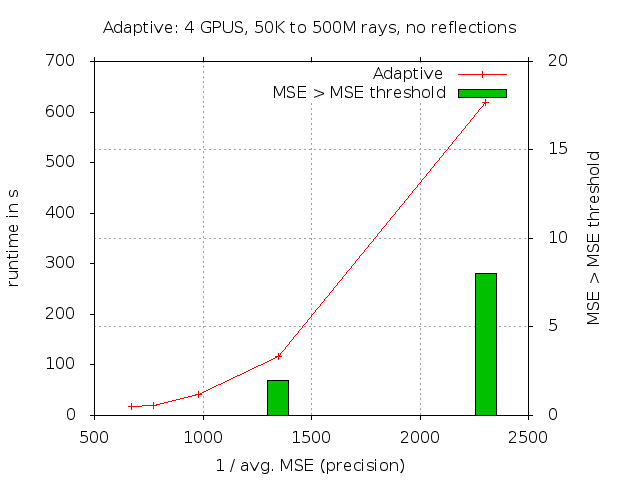
\includegraphics[width=8cm]{plot/adaptive.png}
